% Vertical alignment of columns
\documentclass{ctexbeamer}

% Theme choice:
\usetheme{CambridgeUS}

\begin{document}

\begin{frame}{垂直方向对齐(上部对齐)}
  \begin{columns}[T]
  % Column 1
  \begin{column}{0.5\textwidth}
    This is a neural network with two inputs and two outputs. It has the following parameters:
    \begin{itemize}
      \item Input layer: 2 neurons.
      \item Hidden layer: 5 neurons.
      \item Output layer: 2 neurons.
    \end{itemize}
    The neural network is drawn in \LaTeX{} using Ti\textit{k}Z package. Check latexdraw.com for more details.
  \end{column}
  % Column 2    
  \begin{column}{0.5\textwidth}
    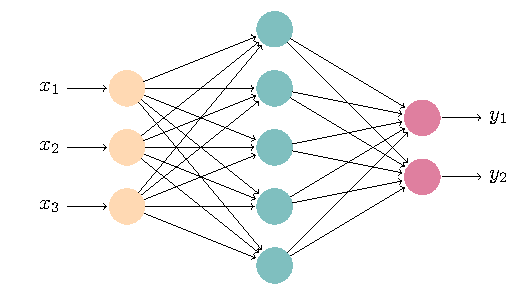
\includegraphics[width=\textwidth]{neural-networks.pdf}
  \end{column}
  \end{columns}
\end{frame}

\end{document}